% Fig. 4.14 -- 兩種自由度的 t 分配畫在完全相同的座標尺度上。
% 書稿來源: mathstatch4.tex 第 5001 至 5035 行的單一個 tikzpicture。
%
% 密度:
%   t(1)  f(x) = 1/(pi (1+x^2))，係數 0.3183098862
%   t(10) f(x) = 0.3891083840 (1 + x^2/10)^(-5.5)，寫成 exp(-5.5 ln(...)) 以免
%         pgfmath 在指數為非整數時失準。
%   兩個界點的右尾機率同為 0.08:
%     t_{0.08}(1)  = 3.894743，該處密度 0.0196864
%     t_{0.08}(10) = 1.517898，該處密度 0.1243979
%   四個數值與書稿一致，已另行以不完全貝塔函數覆核。
%
% 版面: x = 0.75cm、y = 12.9167cm，兩者之比保住書稿 height = 0.625 x width 的比例
%   (x 範圍 12.4、y 範圍 0.45)。書稿以 ymax = 0.45 在峰頂之上留一條空白帶，網頁不留，
%   圖的上緣由圖例決定。
%
% 兩塊尾機率的填色: 書稿把兩塊各以 opacity 0.1 疊著畫，重疊處因而較深。
%   CH2_FIGURE_SPECS.md 1.2 不許以疊加透明度製造層次，故網頁把同一個聯集切成兩塊互不
%   重疊的圖形、同取透明度 0.15:
%     其一 t(10) 曲線之下、x 由 1.517898 到 6 的一塊;
%     其二 t(1) 與 t(10) 兩條曲線之間、x 由 3.894743 到 6 的一塊。
%   兩塊合起來正是「t(10) 的右尾」與「t(1) 的右尾」的聯集，色調均勻。上緣在 x = 3.894743
%   處由 t(10) 跳到 t(1)，那一段跳升就是該處的界線本身。
%
% 兩條曲線依 CH2_FIGURE_SPECS.md 1.9 以線型區分: t(1) 實線、t(10) 為 on 4pt off 2pt。
%   曲線末端無法直接標註 (x = -6 之處兩條相距不到 0.2cm)，故取該節所許的圖例，
%   放在圖內右上角，短線段樣本長 0.5cm。
%
% 字級: 全圖標示一律 \large (12pt)，\DeclareMathSizes{12}{12}{10}{9} 把 script 級撐到
%   10pt。圖內最小的一級是 t 的下標 alpha，即 10pt；沒有 scriptscript。
%   原生尺寸 286.515 x 184.132 pt。S pt 的字在顯示寬 W 之下為 S x 0.99626 x W / 286.515
%   px，故 topic-figure--wide 在手機 350 px 之下 12pt 為 14.60px、10pt 為 12.17px，
%   桌面 620 px 之下為 25.87 / 21.56px。本圖落在 topic-proof 之內，該處手機的可用寬度
%   約 330 px，10pt 仍有 11.47px，守住 11px 的下限。
%   覆核: SVG 內 alpha 的墨跡高 4.50pt，與 tail-identity-f-reciprocal.svg 的 alpha
%   (4.4844pt) 同級，該檔已由數字 1 的 10pt 對 12pt 墨跡比 0.835 確認 script 級為 10pt。
%
% 標示間距: 三個刻度標示的寬度為 0 佔 5.875pt、t_alpha(10) 佔 32.066pt、t_alpha(1) 佔
%   26.191pt。t_alpha(10) 與 t_alpha(1) 相距 0.759cm，合 CH2_FIGURE_SPECS.md 1.3 的
%   0.6cm。0 與 t_alpha(10) 只相距 0.472cm，未達該值: 兩者的間距由 t_{0.08}(10) 這個
%   數值本身決定，只能靠加寬全圖換取，而加寬到 0.6cm 需 x = 0.85cm，原生寬度隨之升到
%   約 315pt，10pt 的字在 330 px 之下跌到 10.5px，破 11px 的下限。字級下限優先，故維持
%   0.472cm；該間距在 350 px 之下仍有 16.4px，是 12pt 字的一又三分之一倍，讀得開。
\documentclass[tikz,border=2pt]{standalone}
\usepackage{amsmath}
\usepackage{amssymb}
\usepackage{xcolor}
\usetikzlibrary{arrows.meta}
\DeclareMathSizes{12}{12}{10}{9}

\definecolor{journalink}{HTML}{1F1C18}
\definecolor{journalmuted}{HTML}{8A7F72}
\definecolor{journalaccent}{HTML}{9C2D2D}

\begin{document}
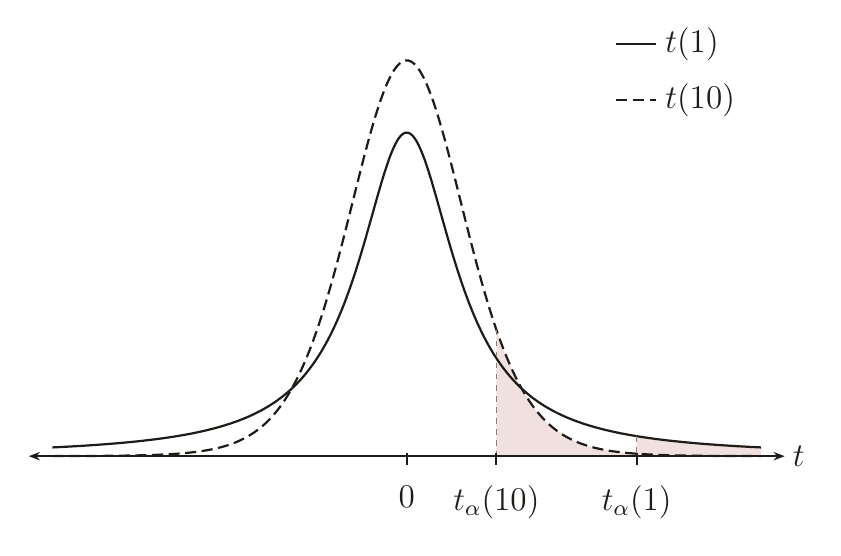
\begin{tikzpicture}[
  x=0.75cm,
  y=12.9167cm,
  every node/.style={font=\large, journalink},
  axis/.style={journalink, line width=0.8pt,
               {Stealth[length=4pt]}-{Stealth[length=4pt]}},
  tick/.style={journalink, line width=0.8pt},
  curveone/.style={journalink, line width=0.8pt},
  curveten/.style={journalink, line width=0.8pt,
                   dash pattern=on 4pt off 2pt},
  guide/.style={journalmuted, line width=0.5pt, dash pattern=on 2pt off 2pt},
  region/.style={journalaccent, fill opacity=0.15}
]

  %% ---- 尾機率的兩塊填色 (互不重疊) -----------------------------------
  % 其一: t(10) 之下，x 由 1.517898 到 6
  \fill[region]
    (1.517898,0) -- (6,0) -- (6,0.0000881)
    -- plot[domain=6:1.517898, samples=160, smooth]
       (\x,{0.3891083840*exp(-5.5*ln(1+\x*\x/10))})
    -- cycle;

  % 其二: t(1) 與 t(10) 之間，x 由 3.894743 到 6
  \fill[region]
    plot[domain=3.894743:6, samples=120, smooth]
       (\x,{0.3891083840*exp(-5.5*ln(1+\x*\x/10))})
    -- plot[domain=6:3.894743, samples=120, smooth]
       (\x,{0.3183098862/(1+\x*\x)})
    -- cycle;

  %% ---- 兩條密度曲線 ---------------------------------------------------
  \draw[curveone] plot[domain=-6:6, samples=300, smooth]
    (\x,{0.3183098862/(1+\x*\x)});
  \draw[curveten] plot[domain=-6:6, samples=300, smooth]
    (\x,{0.3891083840*exp(-5.5*ln(1+\x*\x/10))});

  %% ---- 橫軸 -----------------------------------------------------------
  \draw[axis] (-6.4,0) -- (6.4,0);
  \node[anchor=west, inner sep=2.8pt] at (6.4,0) {$t$};

  %% ---- 兩個界點 -------------------------------------------------------
  \draw[guide] (1.517898,0.1243979) -- (1.517898,0);
  \draw[guide] (3.894743,0.0196864) -- (3.894743,0);
  \foreach \p in {0, 1.517898, 3.894743}
    \draw[tick] ([yshift=0.035cm]\p,0) -- ([yshift=-0.106cm]\p,0);
  \node[anchor=north] at ([yshift=-0.25cm]0,0) {$0$};
  \node[anchor=north] at ([yshift=-0.25cm]1.517898,0) {$t_{\alpha}(10)$};
  \node[anchor=north] at ([yshift=-0.25cm]3.894743,0) {$t_{\alpha}(1)$};

  %% ---- 圖例，右上角 ---------------------------------------------------
  % 短線段樣本由 x = 3.55 到 4.2167 (0.5cm)，文字自 x = 4.37 起。
  % 兩列各在 y = 0.405 與 0.350，兩條曲線在該處都貼著橫軸，不會相碰。
  \draw[curveone] (3.55,0.405) -- (4.2167,0.405);
  \node[anchor=west, inner sep=0pt] at (4.37,0.405) {$t(1)$};

  \draw[curveten] (3.55,0.350) -- (4.2167,0.350);
  \node[anchor=west, inner sep=0pt] at (4.37,0.350) {$t(10)$};

\end{tikzpicture}
\end{document}
